\documentclass[main]{subfiles}

\begin{document}
\setcounter{chapter}{1} %Set chapter counter as week-1
\chapter{More on random walks} %Set chapter name
\setcounter{section}{0}

\lecture{Siva Athreya}{Sanchayan Bhowal, Venkat Trivikram}

\begin{theorem}
    Let $T:\Omega\rightarrow{0,1,\ldots,N}$ be a stopping time. Then,
    $$\E[S_T^2]=E[T].$$
\end{theorem}
\begin{proof}
    $$
        \begin{aligned}
            S_T^2 & =\sum_{k=1}^N S_k^2 \one\{T=k\}                         \\
                  & =\sum_{k=1}^N (S_k^2-S_{k-1}^2) \one\{T\geq k\}         \\
                  & =\sum_{k=1}^N (X_k+S_{k-1})^2-S_{k-1}^2 \one\{T\geq k\} \\
                  & =\sum_{k=1}^N (1+2X_kS_{k-1}) \one\{T\geq k\}.          \\
        \end{aligned}
    $$
    Now, consider $V_k=S_{k-1} \one\{T\geq k\}$. Note that this is a bet sequence. Hence,
    $$
        \begin{aligned}
            \E[S_T^2] & =\E\left[\sum_{k=1}^N\one\{T\geq k\}\right]+2\sum_{k=1}^N\E[X_k V_k] \\
                      & =\sum_{k=1}^N \P(T\geq k)+0                                          \\
                      & =E[T].
        \end{aligned}
    $$
\end{proof}


\section{Reflection Principle}
Assume that $a \in \Z$ and $c>0$. There is a bijection between the paths that cross $a+c$ and those that do not. This bijection is obtained by reflecting the part of the path crossing $a+c$ as shown in the Figure \ref{fig:reflect}. So,
$$\left|S_n=a+c\right|=\left|\sigma_a\leq n \; \& \; S_n=a+c \right|=\left|\sigma_a\leq n \& S_n=a-c \right|$$
Now, we know that all the paths have equal probability. Hence, we get the following lemma.
\begin{lemma}
    $\P(S_n=a+c)=\P(\sigma_a\leq n \; \& \; S_n=a-c)$ where $a \in \Z$ and $c>0$. This is also known as the \emph{reflection principle}.
    \label{lem:reflect}
\end{lemma}
\begin{figure}[ht]
    \label{fig:reflect}
    \centering
    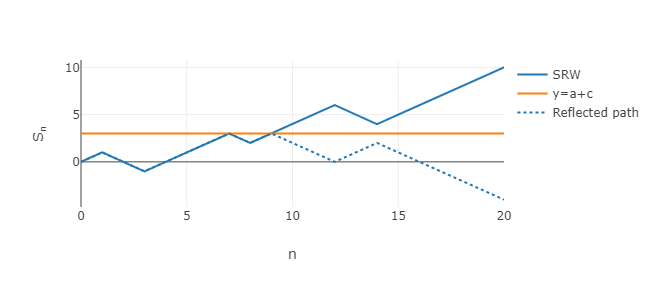
\includegraphics[width=\textwidth]{reflect.png}
    \caption{The figure shows that the bijection between the paths that cross a+c=3 and those that do not.}
\end{figure}
\begin{theorem}
    $\P(\sigma_a\leq n)=\P(S_n\notin [-a,a))$ where $a \in \Z \\ \{0\}$.
\end{theorem}
\begin{proof}
    $$
        \begin{aligned}
            \P(\sigma_a\leq n) & =\P(\sigma_a\leq n, \bigcup_{b \in \Z}{S_n=b} )                                                      \\
                               & =\sum_{b \in \Z} \P(\sigma_a\leq n, S_n=b)                                                           \\
                               & =\sum_{b \in \Z, b\geq a} \P(\sigma_a\leq n, S_n=b)+ \sum_{b \in \Z, b< a} \P(\sigma_a\leq n, S_n=b) \\
                               & =\sum_{b \in \Z, b\geq a} \P(S_n=b)+ \sum_{b \in \Z, b< a} \P(S_n=2a-b)                              \\
                               & =\P(S_n\geq a) + \P(S_n >a)                                                                          \\
                               & =\P(S_n\geq a) + \P(S_n <-a)                                                                         \\
                               & =\P(S_n\notin [-a,a))
        \end{aligned}
    $$
\end{proof}
\begin{corollary}
    $\P(\sigma_a=n)=\frac{1}{2}\left[\P(S_n=a-1)-\P(S_n=a+1)\right]$ where $a \in \Z$.
\end{corollary}
\begin{proof}

\end{proof}
\section{Arc-Sine Law}
Let $L$ denote the last time the random walk hits 0, i.e., $L=\max_{0\leq n \leq 2N} {S_n=0},$ where $N$ denotes the length of the walk.
\begin{theorem}
    $$\P(L=2n)=\frac{1}{2^2N}\binom{2n}{n}\binom{2N-2n}{N-n}.$$
    \label{thm:arcsin}
\end{theorem}
\begin{remark}
    By Stirling's approximation,
    $$\P(L=2n)\sim \frac{1}{\pi N}\frac{1}{\sqrt{\left(\frac{n}{N}\right)\left(1-\frac{n}{N}\right)}}.$$
    $$
        \begin{aligned}
            \P(\frac{L}{2N}\leq x) & =\P(L\leq 2Nx)                                                                         \\
                                   & =\sum_{n=0}^{[2Nx]}\P(L=2n)                                                            \\
                                   & \sim \sum_{n=0}^{[2Nx]} \frac{1}{\pi N}\frac{1}{\sqrt{\left(x\right)\left(1-x\right)}} \\
                                   & \sim \int_{0}^{x}\frac{dy}{pi\sqrt{y(1-y)}}                                            \\
                                   & =\frac{2}{\pi}\sin^{-1}(\sqrt{x}).
        \end{aligned}
    $$
\end{remark}
\begin{proof}[Proof of Theorem \ref{thm:arcsin}]
    Define $\tilde{\sigma_0}\inf\{n: S_n=0, 0< n\le N\}$.
    Consider a path of length $2N$ with $L=2n$. This path can be formed by a path which takes $S_2n=0$ and followed by a path of length $2N-2n$ with $\sigma_0>2N-2n$. Hence, number of paths of length $2N$ with $L=2n$ is the product of the number of paths of length $2n$ with $S_{2n}=0$ and the number of paths of length $2N-2n$ with $\sigma_0>2N-2n$.
    Hence,
    \begin{equation}
        \P(L=2n)=\P(S_{2n}=0)\P(\tilde{\sigma_0}>2N-2n),
        \label{eq:distL}
    \end{equation}
    Now let us compute the distribution of $\tilde{\sigma_0}$.
    \begin{equation}
        \begin{aligned}
            \P(\tilde{\sigma_0}>2k) & =\P(S_1\ne 0, \ldots, S_{2k}\ne 0)                                                           \\
                                    & =2\P(S_1> 0, \ldots, S_{2k}> 0)                                                              \\
                                    & =\frac{2}{2^{2k}} \{\text{No. of paths start at 0 and stay above -1 for }2k-1\text{ steps}\} \\
                                    & =\frac{2}{2^{2k}} \{\text{No. of paths start at 0 and stay below 1 for }2k-1\text{ steps}\}  \\
                                    & =\P(\sigma_1>2k-1)                                                                           \\
                                    & =1-\P(\sigma_1\geq 2k-1)                                                                     \\
                                    & =\P(S_{2k-1}=-1)+\P(S_{2k-1}=0)                                                              \\
                                    & =\P(S_{2k-1}=-1)
        \end{aligned}
        \label{eq:tilds}
    \end{equation}
    Using \eqref{eq:distL} and \eqref{eq:tilds},
    $$
        \begin{aligned}
            \P(L=2n) & =\P(S_{2n}=0)\P(S_{2N-2n-1}=-1)                 \\
                     & =\P(S_{2n}=0)\P(S_{2N-2n}=0)                    \\
                     & = frac{1}{2^2N}\binom{2n}{n}\binom{2N-2n}{N-n}.
        \end{aligned}
    $$
    The first step analysis of $S_2n$ shows that, $\P(S_{2N-2n}=0)=\frac{1}{2}\P(S_{2N-2n-1}=1)+\frac{1}{2}\P(S_{2N-2n-1}=-1)$. Using the symmetry of the walk we know that $\P(S_{2N-2n-1}=1)=\P(S_{2N-2n-1}=-1)$. This gives the second inequality.
\end{proof}
\section{Exercises}
\begin{enumerate}
    \item Complete the proof of Reflection Principle (Lemma \ref{lem:reflect}).
    \item Find the distribution of $M_k=\max_{1\leq k\leq n} S_k$.
\end{enumerate}
\end{document}